\chapter{Introduzione ai Boosted Decsion Tree}

\section{Analisi Multivariata e Problemi di Selezione}
La fisica delle particelle utilizza per i suoi studi acceleratori all'interno dei quali vengono create moltissime particelle. Il problema è quindi quello di individuare le tracce relative ad una specifica particella, che sono in numero molto inferiore rispetto al totale delle particelle create. Diventa, quindi, necessario utilizzare la statistica e il \textit{machine learning} \footnote{machine larning: meccanismo che permette ad una macchina intelligente di migliorare le proprie prestazioni nel tempo. La macchina è in grado di imparare a svolgere determinati compiti migliorando con l'esperienza le proprie capacità \cite{sitoMachineLearning}} può essere un utile mezzo in questo tipo di analisi. Quello che viene spesso fatto è di combinare dei classificatori semplici, che descrivono il problema che si affronta, scelti manualmente in base alle caratteristiche dei dati iniziali. Questo tipo di approccio può dare buoni risultati ma richiede una grande quantità di lavoro e non sempre restituisce risultati ottimali.\cite{articoloDeepLearning} 
\\Il machine learning può essere di tipo supervisionato o non supervisionato. Nel primo caso si utilizzano degli esempi per addestrare l'algoritmo di cui si fornisce anche la "risposta". In questo modo vi è una sorta di feedback su cui si basa l'addestramento. Nel caso non supervisionato, al contrario, vengono forniti solo dei dati e sarà l'algoritmo stesso a decidere indipendentemente come classificarli. L' \textit{analisi multivariata}  appartiene al caso del machine learning supervisionato ed è utilizzata in problemi ad alta dimensionalità. Prevede, infatti, che tutte le variabili vengano combinate (in base al tipo di analisi scelta) in un'unica variabile finale, chiamata \textit{classifier output}, che fornisce il metodo di valutazione finale.
\\In questa tesi si affronta un \textit{problema di selezione}, tipico della fisica delle alte energie (\textit{HEP}, High Energy Physics). In questo caso si parte da una grande quantità di dati iniziali (come milioni di collisioni al secondo) e si vuole identificare un evento raro. Vi è quindi la necessità di migliorare il rapporto tra eventi e background. Spesso si utilizza un trigger iniziale per pre-selezionare i dati di interesse e su questi si va a fare la selezione vera e propria degli eventi. Quest'ultimo passaggio viene risolto individuando la superficie di separazione tra segnale e background. 


    \begin{figure}[htbp]
        \centering
        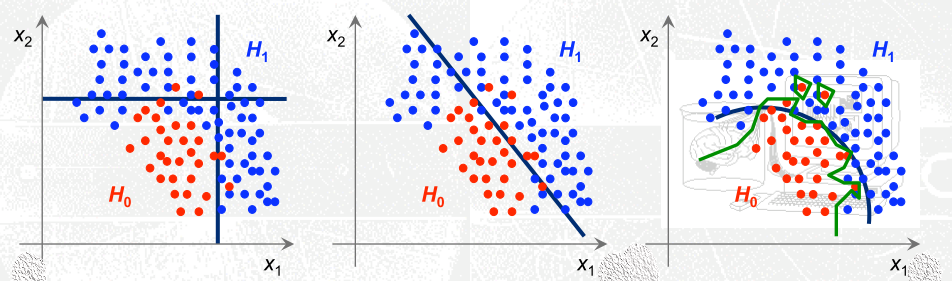
\includegraphics[width=0.8\linewidth]{TMVA/problemiSelezione.png}
        \caption{ Esempi di superdici di separazione tra due classi di eventi.
        \\ Sulla sinistra si sono usati dei tagli rettangolari, al centroun taglio di tipo lineare, mentra a destra un taglio non-lineare }
        \label{fig:esempiCut}
    \end{figure}
    
\section{Boosted Decision Tree}

    \subsection{Decision Tree}
    Un \textit{decision tree} è una struttura che classifica i dati mediante scelte di tipo binario. Se ne riporta un esempio base in figura \ref{fig:BDT}. Ogni scelta è basata su un taglio su una singola variabile.%Devo spiegare cos'è un taglio?
    Ogni ramo creato viene poi nuovamente diviso in due in base al taglio su un'altra variabile. I gruppi di dati creati alla fine dell'albero sono chiamati foglie. Queste vengono selezionate come segnale o background in base alla classe cui appartiene la maggior parte degli eventi. 
    
    \begin{figure}[htbp]
        \centering
        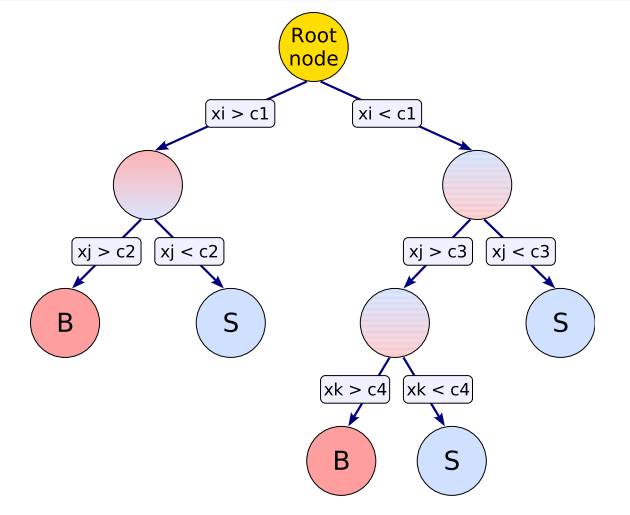
\includegraphics[width=0.5\linewidth]{TMVA/BDT1.PNG}
        \caption{ Esempio di schema di un decision tree}
        \label{fig:BDT}
    \end{figure}
    
    Un vantaggio dei decision tree è che sono facilmente visualizzabili ed è altrettanto semplice ricondursi al significato fisico dei tagli operati. Inoltre sono perlopiù insensibili alla presenza di variabili poco discriminanti (cosa che non accade, invece, per molte altre tecniche di analisi multivariata). Lo svantaggio principale è che sono fortemente sensibili alle fluttuazioni statistiche dei dati utilizzati per il training. Questo problema viene risolto con il "boosting" di cui si parla nella sezione \ref{subsection:Boosting}.
    \\Per poter creare il decision tree serve un set di dati per il \textit{training}, ovvero dei dati di cui si consce già se siano segnale o background. Nel caso della fisica delle alte energie questo viene solitamente realizzato attraverso simulazioni Monte Carlo. La prima divisione dei dati, chiamata root node, viene scelta individuando la variabile e il suo relativo taglio che meglio divide i dati tra segnale e background. L'indice di separazione utilizzato in questa tesi è quello di Gini \footnote{L'indice di Gini è definito come: $p (1-p)$, dove $p$ è la purezza del segnale, che è il rapporto tra il numero di eventi segnale e il numero di eventi totale}. A questo punto si considera singolarmente ognuno dei due rami e si sceglie il taglio sulla variabile che massimizza l'aumento dell'indice di separazione. Si continua così finchè non viene raggiunto uno dei criteri di stop,  a questo punto la struttura dell'albero è formata ed è possibile verificare in che modo sono stati divisi i dati tra segnale e background. 
    \\Infine è necessario fare un controllo per l'\textit{overtraining}, ovvero la possibilità che il decision tree si sia sensibilizzato eccessivamente al set di dati utilizzati nella fase di training e non sia più descrittivo del fenomeno fisico nella sua generalità. Per fare ciò si utilizzano dei dati generati dalla simulazione Monte Carlo, che però non sono stati utilizzati nella fase di training e si controlla che la risposta del decision tree sui dati del training e del testing non differisca troppo.\cite{TMVAGuide} 
 
    \subsection{Boosting}
    Il \textit{boosting} viene utilizzato nel caso dei decision tree, sia per renderli più stabili rispetto alle fluttuazioni statistiche del set di dati del training, sia per migliorarne il rendimento. Per fare ciò si applica il metodo del decision tree molte volte allo stesso set di dati, che però viene pesato in modo diverso ogni volta. 
    \\L'algoritmo di boosting utilizzato in questa tesi è l'\textit{Adaptive Boosting} (AdaBoost). In questo caso i dati che sono stati classificati erroneamente nel precedente decision tree vengono ripesati con un fattore $\aplha$, che è calcolato come 
        \begin{equation}
            \alpha = \frac{1 - err}{err}
        \end{equation}
    Dove $err$ è il rate di eventi classificati erroneamente. 
    \\Si viene a creare una foresta di decision tree da cui si deriva il responso finale per la selezione degli eventi con la formula 
        \begin{equation}
            y = \frac{1}{N_{tot}} \sum_{i=1}^{N_{tot}} {ln(\alpha_i) h_i(x)}
        \end{equation}
    Dove $N_{tot}$ è il numero totale di alberi, e $h(x)$ è il responso del singolo albero.
    Gli algoritmi di boosting funzionano meglio se si utilizzano alberi piccoli,ovvero con pochi livelli di diramazione.
    Utilizzando questa tecnica, pertanto, si riesce a rendere l'algoritmo più stabile ed efficiente ma d'altra parte si perde il senso fisico della selezione tra segnale e background.%spiegare meglio perchè si perde il senso fisico?
    
    
    
    
